\subsection{egui}
egui е проста, бърза и много преносима библиотека за графични потребителски
интерфейси (GUI). Egui работи на много платформи включително: уеб браузъри, като
обикновено приложение и в някои game engine-а. Написана е на Rust и има много
лесен и интуативен API за разработване.

Главните цели на проекта са:
\begin{itemize}
    \item Най-лесната за използване GUI библиотека
    \item Отзивчив: цели поне 60 FPS при компилация с Debug опциите
    \item Преносим: кода да работи в браузър и като собствено приложение
    \item Лесен за интегриране във всяка среда
    \item Разширяем: лесно да пишете свои собствени джаджи за egui
    \item Модулен: можете да използвате малки части от egui и да ги комбинирате
    по нови начини \item Минимален брой завивисимости (библиотеки)
\end{itemize}

\subsubsection{Минимален пример}
egui библиотека ни дава достъп до App интерфейса. Този интерфес съдържа една
функция update. Тя се извиква всеки път когато потребителския интерфейс се е
променил или се получи някакъв евент от мишката или клавиатурата. 
[Фигура \ref{fig:egui-example-1}]

\begin{figure}[!htb]
  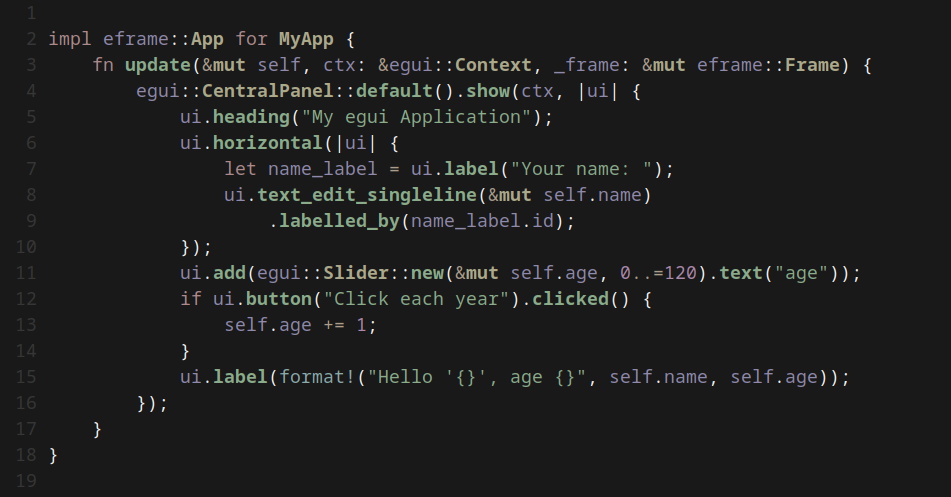
\includegraphics[width=\textwidth,keepaspectratio=true]{egui-example-1}
  \centering
  \caption{Имплементация на egui интерфейса}
  \label{fig:egui-example-1}
\end{figure}

Библиотеката е достатъчно умна сама да прецени дали се нуждае от повторно
изобразяване.

egui е GUI библиотека от незабавен режим (Immediate Mode). Това означава че
начина по който искаме да изглежда графичния интерфейс се описва извиквайки
методи. По този начин се упростява разработката. За да покажем едит прост
бутон се нуждаем от един if оператор.
